
%%%%%%%%%%%%%%%%%%%%%%% file typeinst.tex %%%%%%%%%%%%%%%%%%%%%%%%%
%
% This is the LaTeX source for the instructions to authors using
% the LaTeX document class 'llncs.cls' for contributions to
% the Lecture Notes in Computer Sciences series.
% http://www.springer.com/lncs       Springer Heidelberg 2006/05/04
%
% It may be used as a template for your own input - copy it
% to a new file with a new name and use it as the basis
% for your article.
%
% NB: the document class 'llncs' has its own and detailed documentation, see
% ftp://ftp.springer.de/data/pubftp/pub/tex/latex/llncs/latex2e/llncsdoc.pdf
%
%%%%%%%%%%%%%%%%%%%%%%%%%%%%%%%%%%%%%%%%%%%%%%%%%%%%%%%%%%%%%%%%%%%


\documentclass[runningheads,a4paper]{llncs}

\usepackage{amssymb}
\setcounter{tocdepth}{3}
\usepackage{graphicx}

\usepackage{url}
\newcommand{\keywords}[1]{\par\addvspace\baselineskip
\noindent\keywordname\enspace\ignorespaces#1}

\usepackage{mathtools}
\usepackage{dsfont}
\usepackage{booktabs}
\usepackage{bbold}

\DeclareMathOperator*{\argmin}{arg\,min}
\DeclareMathOperator*{\argmax}{arg\,max}

\usepackage{expl3}
\ExplSyntaxOn
\newcommand\latinabbrev[1]{
  \peek_meaning:NTF . {% Same as \@ifnextchar
    #1\@}%
  { \peek_catcode:NTF a {% Check whether next char has same catcode as \'a, i.e., is a letter
      #1.\@ }%
    {#1.\@}}}
\ExplSyntaxOff

%Omit final dot from each def.
\def\eg{\latinabbrev{e.g}}
\def\etal{\latinabbrev{et al}}
\def\etc{\latinabbrev{etc}}
\def\ie{\latinabbrev{i.e}}
\def\aka{\latinabbrev{a.k.a}}

\newcommand{\Epsilon}{E}

\begin{document}

\mainmatter  % start of an individual contribution

% first the title is needed
\title{Experimental Report on Hyper-parameter Optimization}

% a short form should be given in case it is too long for the running head
\titlerunning{HPO Report}

% the name(s) of the author(s) follow(s) next
%
% NB: Chinese authors should write their first names(s) in front of
% their surnames. This ensures that the names appear correctly in
% the running heads and the author index.
%
\author{\textbf{Xuedong Shang}}
%
\authorrunning{Xuedong Shang}
% (feature abused for this document to repeat the title also on left hand pages)

% the affiliations are given next; don't give your e-mail address
% unless you accept that it will be published
%\institute{Universit\'e de Rennes 1, Parcours MRI \\ \email{xuedong.shang@ens-rennes.fr}}

%
% NB: a more complex sample for affiliations and the mapping to the
% corresponding authors can be found in the file "llncs.dem"
% (search for the string "\mainmatter" where a contribution starts).
% "llncs.dem" accompanies the document class "llncs.cls".
%

\toctitle{}
\tocauthor{Xuedong Shang}
\maketitle


\begin{abstract}

\end{abstract}


\section{Introduction}

The algorithms being considered here for the moment are Hyperband~\cite{li2016}, a Bayesian-based approach TPE~\cite{bergstra2011}, two hierarchical approaches HOO~\cite{bubeck2011}, HCT~\cite{azar2014}, and a baseline method random search. Current datasets used are MNIST dataset and some datasets from UCI machine learning dataset archive.

\section{MNIST}

We consider here Logistic Regression, Multi-Layer Perceptron (MLP) and Convolutional Neural Networks (CNN) as classifiers to be hyper-optimized. This part of code (code for classifers with eventual usage of GPU) is based on code available at \url{http://deeplearning.net/}. 

\paragraph{\textbf{Dataset}} The MNIST dataset is pre-split into three parts: training set $D_{\operatorname{train}}$, validation set $D_{\operatorname{valid}}$ and test set $D_{\operatorname{test}}$.

\paragraph{\textbf{Hyper-parameters}} The hyper-parameters to be optimized are listed below in Table \ref{logistic_sgd}, \ref{mlp_sgd} and \ref{cnn_sgd}. For logistic regression, the hyper-parameters to be considered are learning rate and mini-batch size (since we are doing mini-batch SGD). For MLP, we take into account an additional hyper-parameter which is the $l_2$ regularization factor. For CNN (or LeNet), we take into account the number of kernels used in the two convolutional-pooling layers.

\begin{table}[ht]
\centering
\begin{tabular}{@{}lll@{}}
\toprule
\textbf{Hyper-parameter} & \textbf{Type}                      & \textbf{Bounds}               \\ \midrule
$\operatorname{learning\_rate}$                & $\mathbb{R}^+$ & $\left[ 10^{-3}, 10^{-1} \right]$ (log-scaled) \\
$\operatorname{batch\_size}$           & $\mathbb{N}^+$ & $\left[1, 1000 \right]$         \\ \bottomrule
\end{tabular}
\caption{Hyper-parameters to be optimized for logistic regression with SGD.}
\label{logistic_sgd}
\end{table}

\begin{table}[ht]
\centering
\begin{tabular}{@{}lll@{}}
\toprule
\textbf{Hyper-parameter} & \textbf{Type}                      & \textbf{Bounds}               \\ \midrule
$\operatorname{learning\_rate}$                & $\mathbb{R}^+$ & $\left[ 10^{-3}, 10^{-1} \right]$ (log-scaled) \\
$\operatorname{batch\_size}$           & $\mathbb{N}^+$ & $\left[1, 1000 \right]$         \\ 
$\operatorname{l_2\_reg}$		& $\mathbb{R}^+$ & $\left[ 10^{-4}, 10^{-2} \right]$ (log-scaled) \\ \bottomrule
\end{tabular}
\caption{Hyper-parameters to be optimized for MLP with SGD.}
\label{mlp_sgd}
\end{table}

\begin{table}[ht]
\centering
\begin{tabular}{@{}lll@{}}
\toprule
\textbf{Hyper-parameter} & \textbf{Type}                      & \textbf{Bounds}               \\ \midrule
$\operatorname{learning\_rate}$                & $\mathbb{R}^+$ & $\left[ 10^{-3}, 10^{-1} \right]$ (log-scaled) \\
$\operatorname{batch\_size}$           & $\mathbb{N}^+$ & $\left[1, 1000 \right]$         \\
$\operatorname{k_2}$           & $\mathbb{N}^+$ & $\left[10,  60 \right]$         \\
$\operatorname{k_1}$           & $\mathbb{N}^+$ & $\left[5,  k_2 \right]$         \\ \bottomrule
\end{tabular}
\caption{Hyper-parameters to be optimized for CNN with SGD.}
\label{cnn_sgd}
\end{table}

\paragraph{\textbf{Resource Allocation}} The type of resource considered here is the number of epochs, where one epoch means a pass of training through the whole training set using SGD. Note that this is similar to the original Hyperband paper where one unit of resources corresponds to 100 mini-batch iterations for example. One epoch may contain a various number of mini-batch iterations depending on the mini-batch size.

\paragraph{\textbf{Experimental Design}} In this section, we focus on neural network-typed classifiers, we will thus be maximizing the likelihood of the training set $D_{\operatorname{train}}$ under the model parameterized by $\theta$ (in this section, $\theta$ corresponds to $(W, b)$ where $W$ is the weight matrix and $b$ is the bias vector):
\[
\mathcal{L}(\theta, D_{\operatorname{train}}) = \frac{1}{|D_{\operatorname{train}}|} \sum_i^{|D_{\operatorname{train}}|} \log (\mathbb{P}(Y=y^{(i)}|x^{(i)},\theta),
\]
which is equivalent to minimize the loss function:
\[
\ell(\theta, D_{\operatorname{train}}) = -\mathcal{L}(\theta, D_{\operatorname{train}}).
\]

At each time step $t$, we give one unit of resources (one epoch of training here) to the current algorithm, who will run one epoch of training on the training set $D_{\operatorname{train}}$. The trained model is then used to predict output values $\hat{y}_{\operatorname{pred}}$ and $\tilde{y}_{\operatorname{pred}}$ respectively over validation set $D_{\operatorname{valid}}$ and test set $D_{\operatorname{test}}$. We then compute the number that were misclassified by the model, a.k.a. the zero-one loss on the validation and test set:
\[
\operatorname{valid\_error}_t = \frac{1}{|D_{\operatorname{valid}}|} \sum_i^{|D_{\operatorname{valid}}|} \mathbb{1}_{\{\hat{y}_{\operatorname{pred}}^{(i)} \neq y^{(i)}\}},
\]
\[
\operatorname{test\_error}_t = \frac{1}{|D_{\operatorname{valid}}|} \sum_i^{|D_{\operatorname{valid}}|} \mathbb{1}_{\{\tilde{y}_{\operatorname{pred}}^{(i)} \neq y^{(i)}\}}.
\]

During the experiment, we keep track of the best validation error and its associated test error. At each time step $t$, if the new validation error is smaller than the current best validation error, then we update the best validation error, and report the new test error. Otherwise we just report the test error associated with the previous best validation error.

Note that there is a very important 'keep training' notion here, which means if we are running the classifier with a same hyper-parameter configuration, then we do not restart the training from scratch. In contrary, we always keep track of previously trained weight matrix and bias vector with respect to the current hyper-parameter configuration, and train the model from these pre-trained parameters.

\paragraph{\textbf{Comparison}}
All plots below are averaged on 10 trials of experiments.

\begin{figure}[ht]
    \centering
    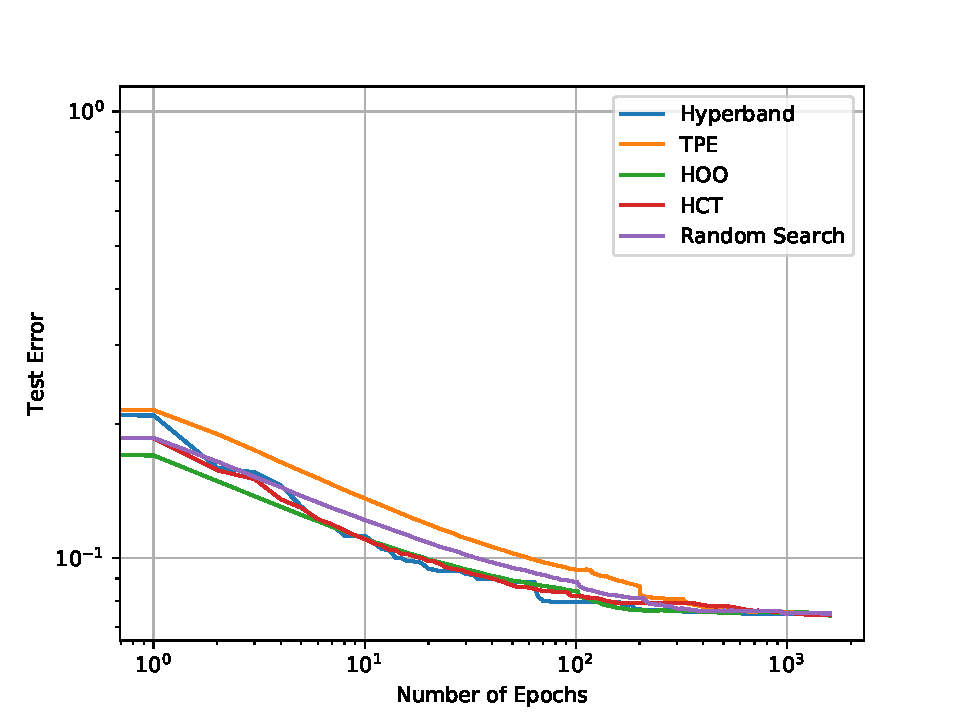
\includegraphics[scale=0.8]{img/mnist/logistic_0.pdf}
    \caption{Performance (log-scale) comparison of different hyper-parameter optimization algorithms on Logistic Regression, trained on MNIST Dataset.}
    \label{logistic_0}
\end{figure}

\begin{figure}[ht]
    \centering
    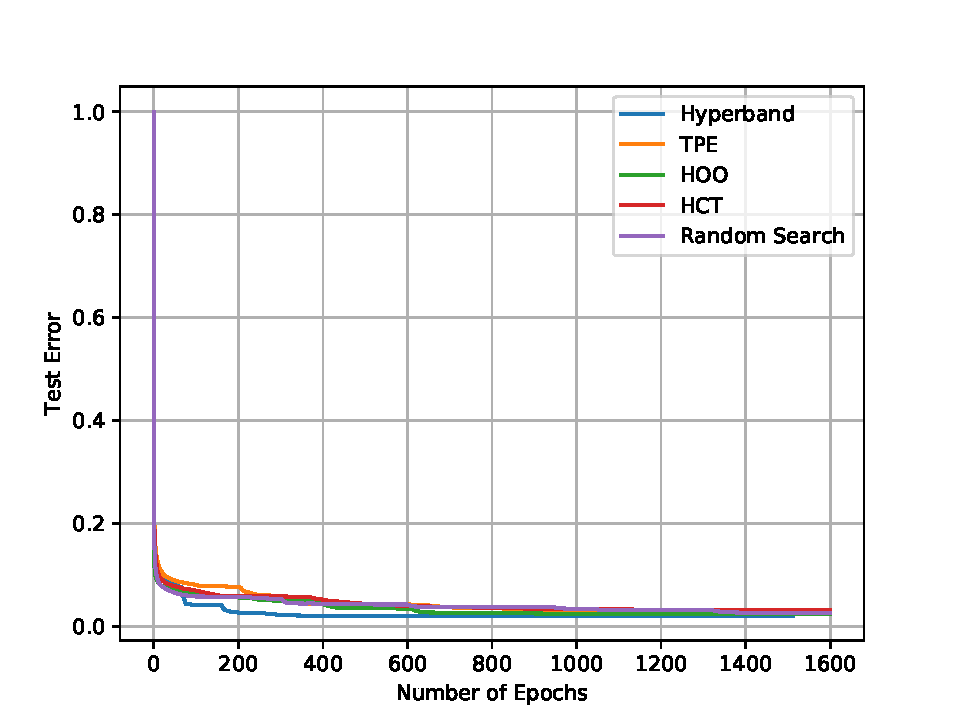
\includegraphics[scale=0.8]{img/mnist/mlp_0.pdf}
    \caption{Performance comparison of different hyper-parameter optimization algorithms on MLP, trained on MNIST Dataset.}
    \label{mlp_0}
\end{figure}

\paragraph{\textbf{Discussion}}


\section{UCI Datasets}

We consider here Support Vector Machine (SVM), Adaptive Boosting (AdaBoost), Gradient Boosting Machine (GBM), Multi-Layer Perceptron (MLP), k-Nearest Neighbors (KNN), Decision Tree and Random Forest.

\paragraph{\textbf{Dataset}} We consider here several datasets on UCI dataset archive (e.g. Wine, Breast Cancer, etc). They are all pre-split into a training set $D_{\operatorname{train}}$ and a test set $D_{\operatorname{test}}$.

\paragraph{\textbf{Hyper-parameters}}

\paragraph{\textbf{Resource Allocation}} One unit of resources in this setting is one iteration of training, which means one complete training of each classifier/regressor over the whole dataset.  

\paragraph{\textbf{Experimental Design}} In this section we use the logarithmic loss, also known as cross-entropy for classification problem, defined by:
\[
\ell(\boldsymbol{y}, \boldsymbol{\hat{p}}) = - \dfrac{1}{n} \sum_{i=1}^n\sum_{j=1}^m y_{ij}\log(\hat{p}_{ij}),
\]
where $\hat{p}_{ij}$ is the predicted probability of a sample $i$ belonging to class $j$, and $m$ is the number of classes considered. And for continuous regression problems, the loss that we use is the typical mean squared error, defined by:
\[
\ell(\boldsymbol{y}, \boldsymbol{\hat{y}}) = \dfrac{1}{n} \sum_i \left(y_i - \hat{y_i}\right)^2
\]

\paragraph{\textbf{Comparison}}

\paragraph{\textbf{Discussion}}

\begin{thebibliography}{4}

\bibitem{li2016} Li, L., Jamieson, K., DeSalvo, G., Rostamizadeh, A., \& Talwalkar, A. (2016). Hyperband: A novel bandit-based approach to hyperparameter optimization. arXiv preprint arXiv:1603.06560.
\bibitem{bergstra2011} Bergstra, J. S., Bardenet, R., Bengio, Y., \& Kégl, B. (2011). Algorithms for hyper-parameter optimization. In Advances in neural information processing systems (pp. 2546-2554).
\bibitem{bubeck2011} Bubeck, S., Munos, R., Stoltz, G., \& Szepesvári, C. (2011). X-armed bandits. Journal of Machine Learning Research, 12(May), 1655-1695.
\bibitem{azar2014} Azar, M. G., Lazaric, A., \& Brunskill, E. (2014). Online stochastic optimization under correlated bandit feedback. In Proceedings of the 31st International Conference on Machine Learning (ICML-14) (pp. 1557-1565).

\end{thebibliography}


%\section*{Appendix}

\end{document}

